\documentclass[First Project.tex]{subfiles}
\begin{document}

\subsection{Πειραματική σύγκριση της ταχύτητας σύγκλισης των τροποιήμενων \\ με τις κλασσικές μεθόδους}

Σε αυτή την παράγραφο γίνεται μία πειραματική σύγκριση μεταξύ τροποποιήμενων και κλασσικών μεθόδων που έχουν υλοποιηθεί στην 
\textbf{1η άσκηση}. Για την σύγκριση αυτή χρησιμοποιούνται δεδομένα από 1000 κλήσεις της κάθε συνάρτησης όπου σε κάθε κλήση μετριέται ο 
χρόνος σε \textlatin{\textbf{ms}} που χρειάστηκε για να τελειώσει ο αλγόριθμος.
\vspace{5mm}
\begin{figure}[h!]
    \centering
    \subfloat{{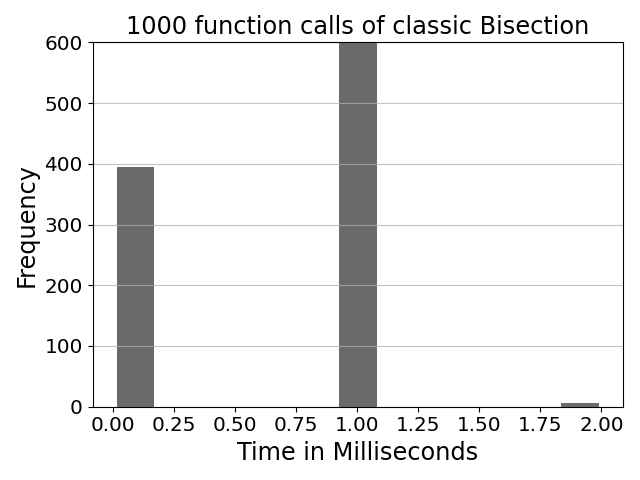
\includegraphics[scale=0.33]{exercise_2_bisection_ms.png}}}
    \quad
    \subfloat{{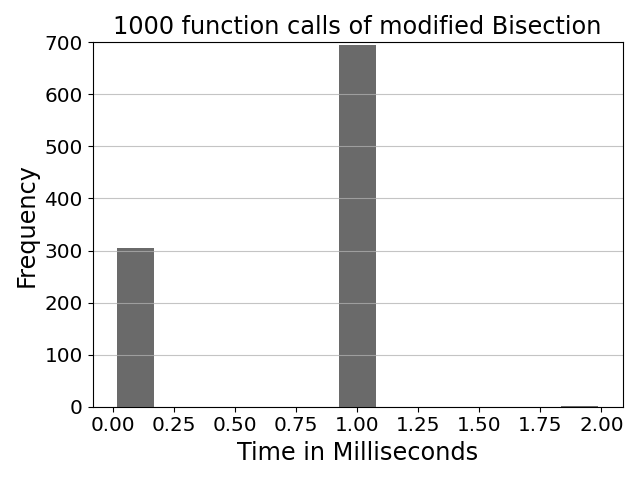
\includegraphics[scale=0.33]{exercise_2_modified_bisection_ms.png}}}
\end{figure}

Από τα παραπάνω ιστογράμματα που αφορούν την μέθοδο της διχοτόμησης παρατηρούμε ότι περίπου 100 παραπάνω κλήσεις της τροποποιήμενης
μεθόδου χρειάζονται 1 \textlatin{\textbf{ms}} σε σχέση με την κλασσική μέθοδο της διχοτόμησης ενώ αντίστοιχα περίπου 100 παραπάνω κλήσεις 
της κλασσικής μεθόδου χρειάζονται μεταξύ 0 και 0.25 \textlatin{\textbf{ms}} σε σχέση με την τροποποιήμενη. Επίσης, παρατηρούμε ότι υπάρχει
ένα μικρό ποσοστό του δείγματος σε κάθε μορφή μεθόδου που χρειάστηκε μεταξύ 1.75 και 2 \textlatin{\textbf{ms}} και αυτό εξάρταται από το μήκος
του διαστήματος με το οποίο κλήθηκε η συνάρτηση. Σε γενικές γραμμές η κλασσική μέθοδος πειραματικά είναι πιο γρήγορη κι αυτό είναι ως ένα
βαθμό λογικό καθώς η τροποποιήμενη εξαρτάται από την ακολουθία των αριθμών που παράγει η συνάρτηση παραγωγής τυχαίων αριθμών.

\vspace{5mm}
\begin{figure}[h!]
    \centering
    \subfloat{{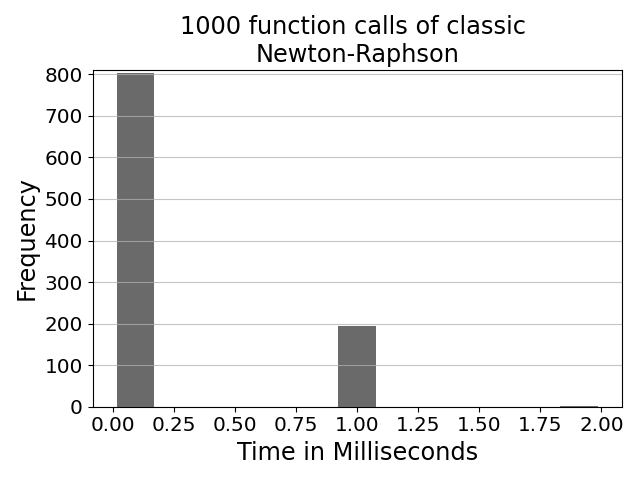
\includegraphics[scale=0.33]{exercise_2_newton_raphson_ms.png}}}
    \quad
    \subfloat{{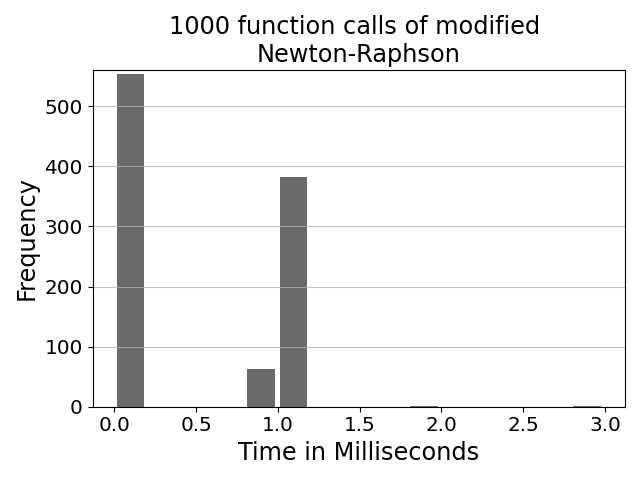
\includegraphics[scale=0.33]{exercise_2_modified_newton_raphson_ms.png}}}
\end{figure}

Από τα παραπάνω ιστογράμματα που αφορούν την μέθοδο \textlatin{Newton-Raphson} παρατηρούμε ότι περίπου 200 παραπάνω κλήσεις της κλασσικής
μεθόδου χρειάστηκαν μεταξύ 0 και 0.25 \textlatin{\textbf{ms}} σε σχέση με την τροποποιήμενη ενώ αντίστοιχα περίπου 200 παραπάνω κλήσεις
της τροποποιήμενης μεθόδου χρειάζονται μεταξύ 1 και 1.5 \textlatin{\textbf{ms}} σε σχέση με την κλασσική. Ακόμα, παρατηρούμε και πάλι ότι
ένα μικρό ποσοστό του δείγματος σε κάθε μορφή μεθόδου χρειάστηκε πάνω από 2 \textlatin{\textbf{ms}} για να ολοκληρωθεί όπου σε αυτή την 
περίπτωση ευθύνεται το αρχικό σημείο. Σε γενικές γραμμές η κλασσική μέθοδος πειραματικά είναι πιο γρήγορη, γεγονός και πάλι λογικό αφού στην
τροποποιήμενη μέθοδο πραγματοποιούνται περισσότερες κλήσεις συναρτήσεων και υπολογίζονται δυνάμεις 2ου και 3ου βαθμού πραγματικών αριθμών.

\vspace{5mm}
\begin{figure}[h!]
    \centering
    \subfloat{{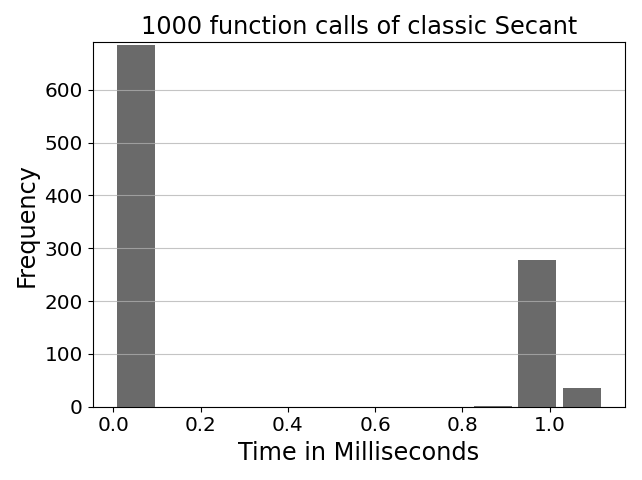
\includegraphics[scale=0.33]{exercise_2_secant_ms.png}}}
    \quad
    \subfloat{{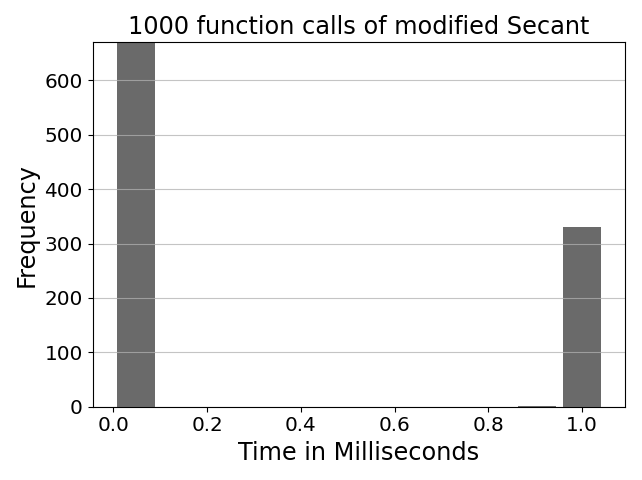
\includegraphics[scale=0.33]{exercise_2_modified_secant_ms.png}}}
\end{figure}

Από τα παραπάνω ιστογράμματα που αφορούν την μέθοδο της τέμνουσας παρατηρούμε ότι οι δύο μέθοδοι αποδίδουν σχεδόν το ίδιο με την κλασσική
μέθοδο να είναι λιγότερο αποδοτική σε περίπου 50 κλήσεις του δείγματος που χρειάστηκε πάνω από 1 \textlatin{\textbf{ms}} σε σχέση 
με την τροποποιήμενη που ήταν πιο σταθερή στην απόδοση της, και πάλι η συμπεριφορά αυτή εξαρτάται από την επιλογή των αρχικών σημείων. Τέλος,
\textbf{τονίζεται} ότι παράλληλα με την εκτέλεση των συναρτήσεων για κάθε μέθοδο το λειτουργικό σύστημα εκτελεί και άλλες διεργασίες που 
μπορεί να επηρρεάσουν την απόδοση του κώδικα, επομένως τα παραπάνω συμπεράσματα και στις τρεις μεθόδους είναι αντιπροσωπευτικά ως ένα βαθμό.
\end{document}